% \setchapterpreamble[u]{\margintoc}
\chapter{Models of type theory}
\labch{models}

Justifying a logic is often achieved using \emph{models}. A model consists
in giving an interpretation to all constructs of the logic we want to study,
such that its rules are still verified.
There are several ways to get models of type theory, I will present some of the
most common ones in this chapter, though my means of choice will be presented in
depth in \nrefch{translations}.

\section{What is a model?}

A model of type theory is an interpretation of the concepts of a type theory
into another theory or object, both living in the same meta-theory.
\begin{figure}[hb]
  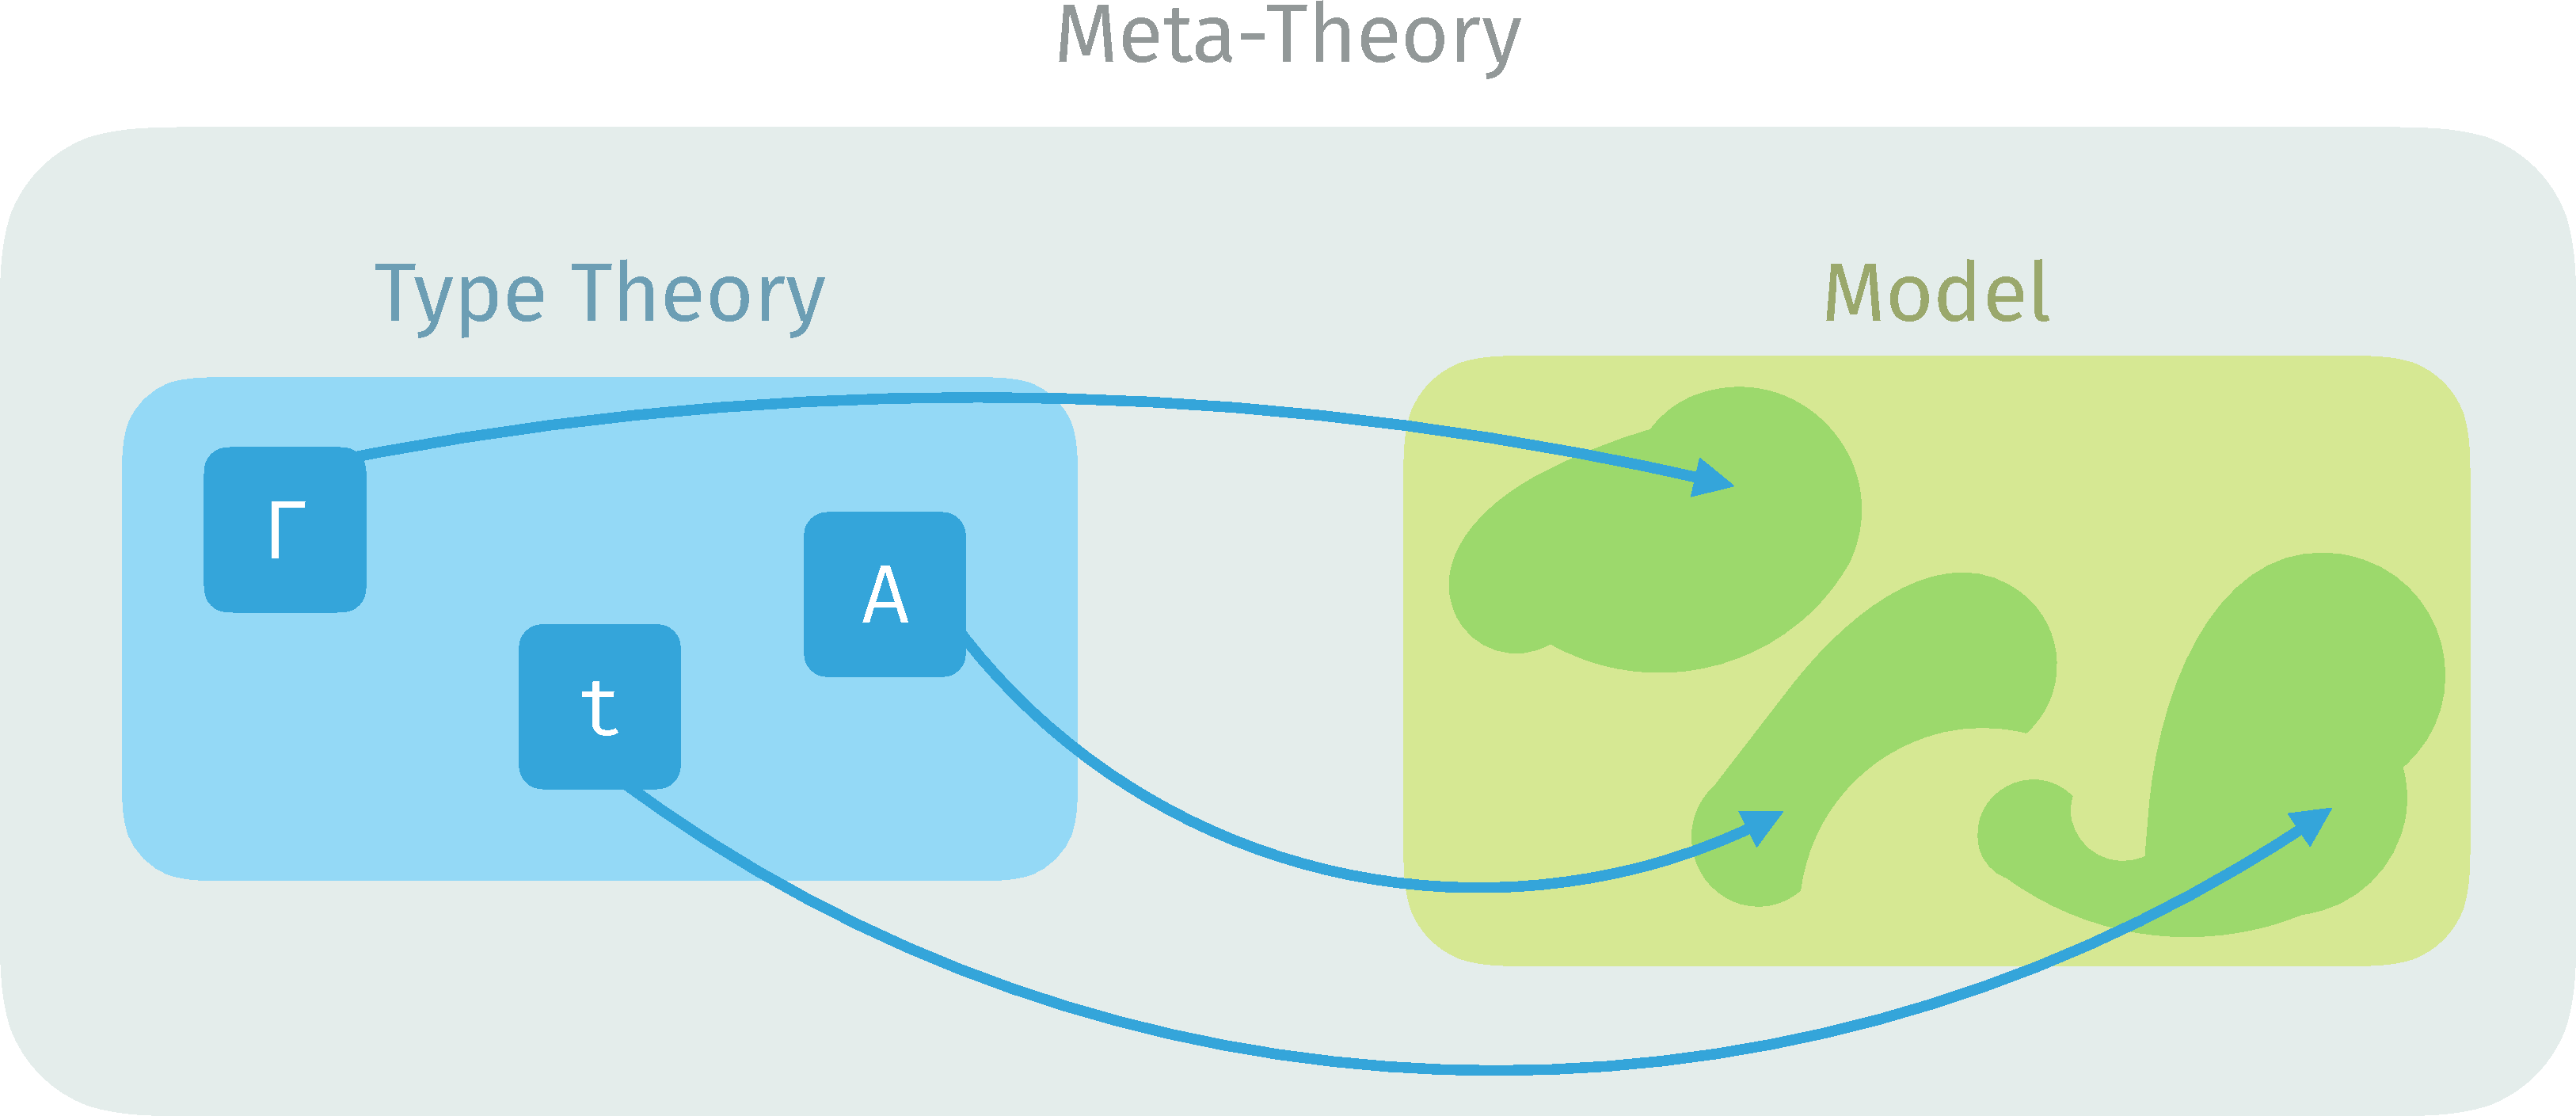
\includegraphics[width=0.9\textwidth]{model}
\end{figure}
To be more precise, a model is given by a class of objects to interpret
contexts, one for terms and one for types; but a model also provides an
interpretation to judgments in such a way that the interpretation is coherent.

\subsection{What can be proved using models}

\paragraph{Consistency.}

I already briefly mentioned this but the main point of models is to prove
consistency of a theory, relying on the already \emph{known} consistency of the
theory in which lives the model... At least in principle. It is however very
rare\sidenote{Impossible?} to \emph{know} that a theory is consistent, instead
we should see it as a theory we \emph{trust}, typically a theory that's widely
accepted as beeing consistent by the community of mathematicians.
This also applies to the meta-theory in which we show that the interpretation is
correct. As such it is best to keep it as simple as possible to avoid relying on
the consistency of too complicated objects.

\paragraph{Independence.}

Another interesting application of models is showing \emph{independence} of a
proposition.

\begin{definition}[Independent proposition]
  A proposition \(P\) is said to be independent from a theory \cT when neither
  \(P\) nor \(\neg P\) can be proven within \cT.
\end{definition}

A way to prove that some \(P\) is independent from \cT is to give a model of \cT
which validates \(P\) and another model which invalidates it (or validates
\(\neg P\)). Indeed if any one of \(P\) or \(\neg P\) %, let us say \(P\),
could be proven in \cT, then it would be valid in both models, leading to
at least one of them being inconsistent.

The fact that a proposition can neither be validated or invalidated in a theory
can come as surprising for some, especially in a classical mindset.
\reminder[-1.8cm]{Classical logic}{
  Classical logic is often characterised by the presence of the \acrshort{LEM}
  which consists in a proof of \(A \vee \neg A\).
}
Gödel's incompleteness theorems have to do with this.

\section{Set-theoretic models}

Set-theoretic models are models of type-theory where types are interpreted as
sets. For instance the (non-dependent) type \(A \to B\) will be interpreted as
the set of set-theoretic functions from the interpretation of \(A\) to the
interpretation of \(B\):
\marginnote[0.55cm]{
  It is usual to write \(\transl{A}\) for the interpretation of \(A\).
}
\[
  \transl{A \to B} \coloneqq \setfun{\transl{A}}{\transl{B}}
\]

Instead of describing all set-theoretic models abstractly I will rather focus on
one example: the proof-irrelevant model of \acrshort{CIC}. I will actually deal
with the smaller case of \acrshort{CoC}.
This is exposed
in~\sidecite[-0.9cm]{miquel2001calcul}---following~\sidecite[-0.3cm]{aczel1998relating,xi2000imperative}---in very clear---and French---way,
but without accounting for contexts and open terms.
I will instead base my own exposition on that of~\sidecite[0.3cm]{werner1997sets},
itself based upon the folklore model seen
in~\sidecite[0.95cm]{coquand1989metamathematical,dybjerinductive,howe1991computational}.
The model is called \emph{proof-irrelevant} because proofs of propositions
(proofs of \(P : \Prop\)) all collapse in the model: provable propositions
are interpreted as the singleton \(\{ \emptyset \}\).

First I will remind what rules we are dealing with. This theory will only have
two universes: \(\Prop\) and \(\Type\), the model can be adapted to deal with
more universes but it is a bit more complicated.
\marginnote[1.7cm]{
  We have two rules for \(\Pi\)-types because we have an impredicative
  universe of propositions \(\Prop\). The rules where \(\Prop\) is on the left
  are unnecessary because we have a weak cumulativity \(\Prop \le \Type\).
}
\marginnote[5.3cm]{
  \(s\) stands for any sort, \ie \(\Prop\) or \(\Type\).
}
\begin{mathpar}
  \infer
    {\vdash \Ga}
    {\Ga \vdash \Prop : \Type}
  %

  \infer
    {\Ga \vdash A : \Prop}
    {\Ga \vdash A : \Type}
  %

  \infer
    {
      \Ga \vdash A : \Type \\
      \Ga, x : A \vdash B : \Type
    }
    {\Ga \vdash \Pi (x:A). B : \Type}
  %

  \infer
    {
      \Ga \vdash A : \Type \\
      \Ga, x : A \vdash B : \Prop
    }
    {\Ga \vdash \Pi (x:A). B : \Prop}
  %

  \infer
    {
      \Ga, x : A \vdash t : B \\
      \Ga \vdash \Pi (x:A). B : s
    }
    {\Ga \vdash \lambda (x:A). t : \Pi (x:A). B}
  %

  \infer
    {
      \Ga \vdash u : \Pi (x:A). B \\
      \Ga \vdash v : A
    }
    {\Ga \vdash u\ v : B[x \sto v]}
  %

  \infer
    {
      \Ga \vdash t : A \\
      \Ga \vdash B : s \\
      A \equiv B
    }
    {\Ga \vdash t : B}
  %
\end{mathpar}
Conversion \(A \equiv B\) is simply the congruent closure of
\(\beta\)-reduction.

As I already said, the idea in this proof-irrelevant model is to interpret
propositions as either the empty set (\(\emptyset\)) for uninhabited
propositions, or as the singleton \(\{ \emptyset \}\) for inhabited ones.
These two sets are the ordinals \(0\) and \(1\) and I will write them as such.
The interpretation of \(\Prop\) is then \(2 \coloneqq \{ 0, 1 \}\).

As you can see in the typing rules we have to deal with terms in a context
\(\Ga\), \ie open terms. The interpretation of such a term is dependent on the
context, this can be easily seen when considering \(x : A \vdash x\)
and \(x : B \vdash x\), the two \(x\) do not necessarily mean the same thing.
As such we will interpret terms together with their context:
\(\transl{\Ga \vdash t}\), which will be set-theoretic functions of domain
\(\transl{\Ga}\), without a precise codomain.

\(\transl{\Ga}\) is defined as follows:
\[
  \begin{array}{rcl}
    \transl{\ctxempty} &\coloneqq& 1 \\
    \transl{\Ga, x:A} &\coloneqq&
    \{
      (\gamma, a) \mid
      \gamma \in \transl{\Ga} \wedge a \in \transl{\Ga \vdash A}(\gamma)
    \}
  \end{array}
\]
mutually with \(\transl{\Ga \vdash t}\):
\sidedef[-0.5cm]{Dependent product of sets}{
  \(\prod_{x \in A} B(x)\) is defined as the set of functions \(f\) from \(A\)
  to \(\bigcup_{x \in A} B(x)\) such that \(f(x) \in B(x)\).
}
\[
  \begin{array}{rcl}
    \transl{\Ga \vdash \Pi (x:A). B}(\gamma)
    &\coloneqq&
    \prod_{a \in \transl{\Ga \vdash A}(\gamma)}\
    \transl{\Ga, x:A \vdash B}(\gamma, a) \\
    \transl{\Ga \vdash \Prop}(\gamma) &\coloneqq& 2 \\
    \transl{\Ga \vdash \Type}(\gamma) &\coloneqq& \mathcal{U} \\
    \transl{\Ga \vdash \lambda (x:A). t}(\gamma)
    &\coloneqq&
    a \in \transl{\Ga \vdash A}(\gamma) \mapsto
    \transl{\Ga, x:A \vdash t}(\gamma,a) \\
    \transl{\Ga \vdash u\ v}(\gamma) &\coloneqq&
    \transl{\Ga \vdash u}(\gamma)(\transl{\Ga \vdash v}(\gamma)) \\
    \transl{\Ga \vdash x_i}(\gamma) &\coloneqq& \pi_2 \circ \pi_1^i (\gamma)
  \end{array}
\]
where in the last equality
\[
  \Ga = x_n : A_n, \dots x_i : A_i, \dots x_0 : A_0
\]
I do not really believe you can distinguish between propositions and usual types
in the current setting so in~\sidecite{aczel1998relating}, Aczel introduces a
non-standard encoding of set-theoretic functions such that the constant function
\(x \mapsto 0\) is \emph{equal} to \(0\).

I did not precise what \(\mathcal{U}\) was. From \(\mathcal{U}\) we only require
that it is closed under product and power-sets and contains at least \(2\).
It needs only be the cardinal \(\aleph_0\) in our case, but if we wanted more
universes---say a hierarchy of them---we could use inaccessible cardinals.
We will see them briefly in \refsec{cat-models}.

Before we can claim it is a model we need to show that whenever
\(\Ga \vdash t : A\) then \(\transl{\Ga \vdash t} \in \transl{\Ga \vdash A}\).
This will in particular prove that every proof of a proposition is indeed sent
to \(0\).
It also allows us to conclude consistency since the empty type
\[
  \bot \coloneqq \Pi (P : \Prop). P
\]
is interpreted (in the empty context) as
\[
  \transl{\vdash \bot}(0) = \prod_{X \in 2}\ X
\]
\ie the set of functions \(f\) such that \(f(0) \in 0\) and \(f(1) \in 1\),
since there is no element in \(0\) there is no such \(f\) and as such
\[
  \transl{\vdash \bot} = 0
\]

The proof is done by looking at each rule and showing they preserve the
property: for instance if we take
\[
  \infer
    {
      \Ga, x : A \vdash t : B \\
      \Ga \vdash \Pi (x:A). B : \Type
    }
    {\Ga \vdash \lambda (x:A). t : \Pi (x:A). B}
  %
\]
we assume we have
\(\transl{\Ga, x:A \vdash t}(\delta) \in \transl{\Ga, x:A \vdash B}(\delta)\)
and
\(\transl{\Ga \vdash \Pi (x:A). B}(\gamma) \in \transl{\Ga \vdash \Type}(\gamma)\)
for every \(\delta \in \transl{\Ga, x:A}\) and \(\gamma \in \transl{\Ga}\)
and show that
\[
  \transl{\Ga \vdash \lambda (x:A). t}(\gamma) \in
  \transl{\Ga \vdash \Pi (x:A). B}(\gamma)
\]
If we reformulate we want to show that for all \(\gamma \in \Ga\) and
\(a \in \transl{\Ga \vdash A}(\gamma)\) we have
\[
  \transl{\Ga, x : A \vdash t}(\gamma, a) \in
  \transl{\Ga, x:A \vdash B}(\gamma,a)
\]
which corresponds to our hyothesis.

For some other cases like the conversion and application rules we need to show
that convertible terms are sent to equal sets/functions and that the
interpretation behaves well with respect to substitution.
I will not dwell on the details as it has been dealt with nicely in the
references I put at the beginning of this section.

Set-theoretic models are not the only way to make models of type theory of
course. For instance they may not be best-suited to interpretation of
computational content since \(\beta\)-convertible terms are interpreted as the
same set. They however provide a nice way of seeing the relation between
set-theory---the widely accepted framework in which to do mathematics---and type
theory which we\sidenote{I'll leave that one as imprecise as it is.} advocate
instead.

\section{Categorical models}
\labsec{cat-models}

Categorical models are one of the most used way of defining models for type
theories. There are several notions of categorical models:
contextual categories~\sidecite[-0.9cm]{cartmell1986generalised} from which stem
categories with attributes~\sidecite[0.2cm]{hofmann1994interpretation} and
C-systems~\sidecite[0.9cm]{voevodsky2016subsystems},
\acrfullpl{CwF}~\sidecite[1.7cm]{dybjer1995internal}, and more...
I will focus on \acrshortpl{CwF} in this document.

\subsection{Categories with families}

A \acrshort{CwF} is given by
\begin{enumerate}
  \item a collection of objects (or contexts) \(\Con\);
  \item morphisms (or substitutions) \(\sigma : \Ga \to \D\) between contexts
  \(\Ga, \D : \Con\);
  \item for each context \(\Ga : \Con\), a collection \(\CTy\ \Ga\) of types in
  that context;
  \item for each context \(\Ga : \Con\) and type \(A : \CTy\ \Ga\), a collection
  \(\CTm\ \Ga\ A\) of terms of type \(A\);
  \item an operation of substitution for types taking \(\sigma : \Ga \to \D\)
  and a type \(A : \CTy\ \D\) to type \(A[\sigma] : \CTy\ \Ga\);
  \item \label{item:term-subst} a similar substitution operation on terms taking
  \(\sigma : \Ga \to \D\) and a term \(t : \CTm\ \D\ A\) to term
  \(t[\sigma] : \CTm\ \Ga\ A[\sigma]\);
  \item a terminal object representing the empty context \(\ctxempty : \Con\);
  \item an extension operation taking \(\Ga : \Con\) and \(A : \CTy\ \Ga\)
  to a new object \(\Ga, A : \Con\) together with a morphism
  \(\pp : \Ga, A \to \Ga\) and a term \(\pq : \CTm\ (\Ga, A)\ A[\pp]\);
  \item an operation taking \(\sigma : \Ga \to \D\) and term
  \(a : \CTm\ \Ga\ A[\sigma]\) to substitution \(\sigma, a : \Ga \to \D, A\)
  such that \(\pp \circ (\sigma, a) = \sigma\) and \(\pq[\sigma, a] = a\).
\end{enumerate}
The two first have to give the structure of category, this in particular means
that there is an identity substitution, and associative composition of those.

The category \(\Set\) of sets is a \acrshort{CwF}:
\marginnote[3.8cm]{
  \ref{item:term-subst} holds because for every \(\gamma \in \Ga\),
  \[
    (t \circ \sigma)(\gamma) = t(\sigma(\gamma)) \in A_{\sigma(\gamma)}
    = A[\sigma]_\gamma
  \]
}
\begin{enumerate}
  \item objects are sets;
  \item substitutions are given as set-theoretic functions, composed as
  functions;
  \item types in \(\CTy\ \Ga\) are sets indexed by \(\Ga\);
  \item terms of \(\CTm\ \Ga\ A\) are choice functions
  \(t \in \setfun{\Ga}{\bigcup_{\gamma \in \Ga} A_\gamma}\) such that
  \(t(\gamma) \in A_\gamma\) for every \(\gamma \in \Ga\);
  \item given \(\sigma : \Ga \to \D\) and \(A : \CTy\ \D\), \(A[\sigma]\)
  is defined as the \(\Ga\)-indexed family \((A_{\sigma(\gamma)})_\gamma\);
  \item given \(\sigma : \Ga \to \D\) and \(t : \CTm\ \D\ A\), \(t[\sigma]\)
  is defined as the choice function \(t \circ \sigma\);
  \item the empty context is given as the singleton \(\{ \emptyset \}\);
  \item given \(\Ga : \Con\) and \(A : \CTy\ \Ga\), \(\Ga, A\) is defined as
  the disjoint union \(\amalg_{\gamma \in \Ga} A_\gamma\), \(\pp\) and \(\pq\)
  are defined as the first and second projection respectively;
  \item given \(\sigma : \Ga \to \D\) and \(a : \CTm\ \Ga\ A[\sigma]\),
  \(\sigma, a\) is defined as the function
  \(\gamma \mapsto (\sigma(\gamma), a(\gamma))\) which verifies the conditions.
\end{enumerate}

Right now this only interprets a type theory with no type or term constructors.
I will give a few example of those.

\paradot{Dependent products}

A \acrshort{CwF} is said to have dependent products when it has the following
elements:
\begin{itemize}
  \item for any \(A : \CTy\ \Ga\) and \(B : \CTy\ (\Ga, A)\) there exists
  \(\Pi\ A\ B : \CTy\ \Ga\);
  \item for \(b : \CTm\ (\Ga, A)\ B\) there exists
  \(\lambda b : \CTm\ \Ga\ (\Pi\ A\ B)\);
  \item for \(f : \CTm\ \Ga\ (\Pi\ A\ B)\) and \(u : \CTm\ \Ga\ A\) there exists
  \(\capp(f,u) : \CTm\ \Ga\ B[\cid, u]\)
\end{itemize}
such that for any \(\sigma : \D \to \Ga\) and terms and types as above the
following equations hold:
\[
  \begin{array}{rcl}
    (\Pi\ A\ B)[\sigma] &=& \Pi\ A[\sigma]\ B[(\sigma \circ \pp), \pq] \\
    (\lambda b)[\sigma] &=& \lambda b[(\sigma \circ \pp), \pq] \\
    (\capp(f,u))[\sigma] &=& \capp(f[\sigma],u[\sigma]) \\
    \capp(\lambda b, u) &=& b[\cid, u] \\
    \lambda \capp(f[\pp], \pq) &=& f
  \end{array}
\]

\sidedef[-0.7cm]{\(\eta\)-expansion}{
  \(\eta\)-expansion is defined as follows
  \[
    t \red_\eta \lambda x.\ t\ x
  \]
  \(\eta\)-contraction is the opposite relation.
}
The first four equations are simply there to attest to the good behaviour of
substitution. The last two are more interesting, corresponding to
\(\beta\)-reduction and \(\eta\)-contraction respectively.

\paradot{Dependent sums}

A \acrshort{CwF} has (negative) dependent sums
when:
\marginnote{
  See \nrefch{flavours} for a discussion on negative vs positive sums.
}
\begin{itemize}
  \item for any \(A : \CTy\ \Ga\) and \(B : \CTy\ (\Ga, A)\) there exists
  \(\Sigma\ A\ B : \CTy\ \Ga\);
  \item for \(a : \CTm\ \Ga\ A\) and \(b : \CTm\ \Ga\ B[\cid,a]\) there exists
  the dependent pair \(\dpair{a,b} : \CTm\ \Ga\ (\Sigma\ A\ B)\);
  \item for \(p : \CTm\ \Ga\ (\Sigma\ A\ B)\) there exists
  \(p.1 : \CTm\ \Ga\ A\);
  \item for \(p : \CTm\ \Ga\ (\Sigma\ A\ B)\) there exists
  \(p.2 : \CTm\ \Ga\ B[\cid, p.1]\)
\end{itemize}
such that
\[
  \begin{array}{rcl}
    (\Sigma\ A\ B)[\sigma] &=& \Sigma\ A[\sigma]\ B[(\sigma \circ \pp), \pq] \\
    \dpair{a,b}[\sigma] &=& \dpair{a[\sigma], b[\sigma]} \\
    (p.1)[\sigma] &=& p[\sigma].1 \\
    (p.2)[\sigma] &=& p[\sigma].2 \\
    \dpair{a,b}.1 &=& a \\
    \dpair{a,b}.2 &=& b
  \end{array}
\]

\paradot{Identity types}

A \acrshort{CwF} has identity types---another name for the equality type---when:
\begin{itemize}
  \item for \(A : \CTy\ \Ga\) and \(u, v : \CTm\ \Ga\ A\) there exists
  \(\CId_A\ u\ v : \CTy\ \Ga\);
  \item for \(A : \CTy\ \Ga\) and \(u : \CTm\ \Ga\ A\) there exists
  \(\crefl_u : \CTm\ \Ga\ (\CId_A\ u\ u)\)
\end{itemize}
such that
\[
  \begin{array}{rcl}
    (\CId_A\ u\ v)[\sigma] &=& \CId_{A[\sigma]}\ u[\sigma]\ v[\sigma] \\
    (\crefl_a)[\sigma] &=& \crefl_{a[\sigma]}
  \end{array}
\]
In a lot of models, equality ends up being interpreted as the equality of the
model meaning the eliminator is not necessary, hence my not requiring it.
Models that deal with equality differently are of course interesting but I
will keep things simple in this chapter.

\paradot{Booleans}

A \acrshort{CwF} has booleans when for any \(\Ga : \Con\) it has
\begin{itemize}
  \item \(\bool : \CTy\ \Ga\);
  \item \(\ttrue : \CTm\ \Ga\ \bool\);
  \item \(\ffalse : \CTm\ \Ga\ \bool\);
  \item given \(b : \CTm\ \Ga\ \bool\), \(C : \CTy\ (\Ga, \bool)\),
  \(t : \CTm\ \Ga\ C[\cid, \ttrue]\) and \(f : \CTm\ \Ga\ C[\cid, \ffalse]\),
  some \(\tif{b}{C}{t}{f} : \CTm\ \Ga\ C[\cid, b]\)
\end{itemize}
such that
\[
  \begin{array}{rcl}
    \bool[\sigma] &=& \bool \\
    \ttrue[\sigma] &=& \ttrue \\
    \ffalse[\sigma] &=& \ffalse \\
    \left(\fitif{b}{C}{t}{f}\right)[\sigma] &=&
    \fitif{b[\sigma]}{C[(\sigma \circ \pp), \pq]}{t[\sigma]}{f[\sigma]} \\
    \tif{\ttrue}{C}{t}{f} &=& t \\
    \tif{\ffalse}{C}{t}{f} &=& f
  \end{array}
\]

\paradot{Natural numbers}

A \acrshort{CwF} has natural numbers when, given \(\Ga : \Con\), it has
\begin{itemize}
  \item \(\nat : \CTy\ \Ga\);
  \item \(\czero : \CTm\ \Ga\ \nat\);
  \item for \(n : \CTm\ \Ga\ \nat\), \(\csucc\ n : \CTm\ \Ga\ \nat\);
  \item for \(n : \CTm\ \Ga\ \nat\), \(C : \CTy\ (\Ga, \nat)\),
  \(z : \CTm\ \Ga\ C[\cid, \czero]\) and
  \(s : \CTm\ \Ga\ (\Pi\ \nat\ \Pi\ C\ C[(\pp, \csucc\ \pq) \circ \pp])\),
  there exists \(\natrec_C\ n\ z\ s : \CTm\ \Ga\ C[\cid, n]\)
\end{itemize}
\marginnote[-1.3cm]{
  For the successor I use \(\Pi\)-types when I could have instead put things
  in the context. Both are valid and I'm often favorable to the idea that things
  should be kept separate as much as possible, but the reliance on application
  and everything allows us to avoid proving the same things several times,
  especially since manipulating contexts is so tedious with categories.
}
such that
\[
  \begin{array}{rcl}
    \nat[\sigma] &=& \nat \\
    \czero[\sigma] &=& \czero \\
    (\csucc\ n)[\sigma] &=& \csucc\ n[\sigma] \\
    (\natrec_C\ n\ z\ s) &=&
    \natrec_{C[(\sigma \circ \pp), \pq]}\ n[\sigma]\ z[\sigma]\ s[\sigma] \\
    \natrec_C\ \czero\ z\ s &=& z \\
    \natrec_C\ (\csucc\ n)\ z\ s &=& \capp(\capp(s,n), \natrec_C\ n\ z\ s)
  \end{array}
\]

\paradot{Tarski universes}

A Tarski universe is given by
\begin{itemize}
  \item a type \(\CU : \CTy\ \Ga\);
  \item for \(a : \CTm\ \Ga\ \CU\), a type \(\CEl(a) : \CTy\ \Ga\);
  \item for \(a : \CTm\ \Ga\ \CU\), \(b : \CTm\ \Ga\ (\Pi\ \CEl(a)\ \CU)\),
  a term \(\pi(a,b) : \CTm\ \Ga\ \CU\)
\end{itemize}
such that
\[
  \begin{array}{rcl}
    \CU[\sigma] &=& \CU \\
    \CEl(a)[\sigma] &=& \CEl(a[\sigma]) \\
    \CEl(\pi(a,b)) &=& \Pi\ \CEl(a)\ \CEl(\capp(b[\pp], \pq))
  \end{array}
\]
This makes the universe closed under dependent types, we can of course extend
this notion to include other constructions.

All of these can be defined in the \(\Set\) model above. They are however all
simpler cases than the \(\Card\) model I will give in the next section so I
will not detail them.

\subsection{Cardinal model}
\labsubsec{card-model}

In the previous section I briefly presented the \(\Set\) model. Here I will
detail the cardinal model of type theory that we initially wrote with Andrej
Bauer. It teaches us interesting things about syntax and especially about
\acrshort{ETT}.

\marginnote[0.1cm]{
  The existence of such a bijection and this definition of cardinal relies on
  the axiom of choice. This is not constructive at all.
}
For every set \(X\) there is a unique cardinal \(\card{X}\) such that
\(X \cong \card{X}\). We choose a bijection \(\beta_X : \setfun{X}{\card{X}}\).
I will write \(\beta\) for \(\beta_X\) when the \(X\) is understood.

The \(\Card\) \acrshort{CwF} is defined very similarly to \(\Set\):
\begin{enumerate}
  \item objects are cardinals;
  \item substitutions are given as set-theoretic functions, composed as
  functions;
  \item types in \(\CTy\ \Ga\) are cardinals indexed by \(\Ga\);
  \item terms of \(\CTm\ \Ga\ A\) are choice functions
  \(t \in \setfun{\Ga}{\bigcup_{\gamma \in \Ga} A_\gamma}\) such that
  \(t(\gamma) \in A_\gamma\) for every \(\gamma \in \Ga\);
  \item given \(\sigma : \Ga \to \D\) and \(A : \CTy\ \D\), \(A[\sigma]\)
  is defined as the \(\Ga\)-index family \((A_{\sigma(\gamma)})_\gamma\);
  \item given \(\sigma : \Ga \to \D\) and \(t : \CTm\ \D\ A\), \(t[\sigma]\)
  is defined as the choice function \(t \circ \sigma\);
  \item the empty context is given as the cardinal \(1\);
  \item given \(\Ga : \Con\) and \(A : \CTy\ \Ga\), \(\Ga, A\) is defined as
  the cardinal of the disjoint union
  \(\card{\amalg_{\gamma \in \Ga} A_\gamma}\), \(\pp\) is defined as
  \(\pi_1 \circ \beta^{-1}\) where \(\pi_1\) is the first projection of the
  disjoint union, \(\pq\) is defined as \(\pi_2 \circ \beta^{-1}\);
  \item given \(\sigma : \Ga \to \D\) and \(a : \CTm\ \Ga\ A[\sigma]\),
  \(\sigma, a\) is defined as the function
  \(\gamma \mapsto \beta(\sigma(\gamma), a(\gamma))\).
\end{enumerate}

Let us verify the coherence conditions:
\[
  \begin{array}{rcl}
    \pp \circ (\sigma, a) &=& \sigma \\
    \pq [\sigma, a] &=& a
  \end{array}
\]
\marginnote[0.8cm]{
  Notice how I verify equality of functions extensionally, that is because we
  are considering set-theoretic functions here.
}
Given \(\sigma : \Ga \to \D\), \(a : \CTm\ \Ga\ A[\sigma]\) and
\(\gamma \in \Ga\) we have
\[
  \begin{array}{lclcl}
    (\pp \circ (\sigma, a))(\gamma) &=&
    \pp((\sigma, a)(\gamma)) \\
    &=& \pp(\beta(\sigma(\gamma),a(\gamma))) \\
    &=& (\pi_1 \circ \beta^{-1})(\beta(\sigma(\gamma),a(\gamma))) \\
    &=& \pi_1(\beta^{-1}(\beta(\sigma(\gamma),a(\gamma)))) \\
    &=& \pi_1(\sigma(\gamma), a(\gamma)) &=& \sigma(\gamma)
  \end{array}
\]
and
\[
  \begin{array}{lclcl}
    (\pq [\sigma, a])(\gamma) &=&
    (\pq \circ (\sigma, a))(\gamma) \\
    &=& \pq((\sigma,a)(\gamma)) \\
    &=& \pq(\beta(\sigma(\gamma),a(\gamma))) \\
    &=& (\pi_2 \circ \beta^{-1})(\beta(\sigma(\gamma),a(\gamma))) \\
    &=& \pi_2(\beta^{-1}(\beta(\sigma(\gamma),a(\gamma)))) \\
    &=& \pi_2(\sigma(\gamma),a(\gamma)) &=& a(\gamma)
  \end{array}
\]

I will now echo the previous section and show that \(\Card\) admits all the
constructions I introduced then.

\paradot{Dependent products}

Given \(A : \CTy\ \Ga\) and \(B : \CTy\ (\Ga, A)\) we define
\(\Pi\ A\ B : \CTy\ \Ga\) as
\[
  (\Pi\ A\ B)(\gamma) \coloneqq \card{\prod_{x \in A(\gamma)} B(\beta(\gamma,x))}
\]
We define abstraction and application as follows:
\marginnote[0.7cm]{
  With \(b : \CTm\ (\Ga,A)\ B\), \(f : \CTm\ \Ga\ (\Pi\ A\ B)\) and
  \(u : \CTm\ \Ga\ A\).
}
\[
  \begin{array}{lcl}
    (\lambda b)(\gamma) &\coloneqq& \beta(x \mapsto b(\beta(\gamma,x))) \\
    \capp(f,u)(\gamma) &\coloneqq& \beta^{-1}(f(\gamma))(u(\gamma))
  \end{array}
\]
Now we show
\[
  \begin{array}{rcl}
    (\Pi\ A\ B)[\sigma] &=& \Pi\ A[\sigma]\ B[(\sigma \circ \pp), \pq] \\
    (\lambda b)[\sigma] &=& \lambda b[(\sigma \circ \pp), \pq] \\
    (\capp(f,u))[\sigma] &=& \capp(f[\sigma],u[\sigma]) \\
    \capp(\lambda b, u) &=& b[\cid, u] \\
    \lambda \capp(f[\pp], \pq) &=& f
  \end{array}
\]

\[
  \begin{array}{rcl}
    (\Pi\ A[\sigma]\ B[(\sigma \circ \pp), \pq])(\gamma)
    &=& \card{
      \prod_{x \in A[\sigma](\gamma)}
      B[(\sigma \circ \pp), \pq](\beta(\gamma, x))
    } \\
    &=& \card{
      \prod_{x \in A(\sigma(\gamma))}
      B(((\sigma \circ \pp), \pq)(\beta(\gamma, x)))
    } \\
    &=& \card{\prod_{x \in A(\sigma(\gamma))} B(\beta(\sigma(\gamma),x))} \\
    &=& (\Pi\ A\ B)(\sigma(\gamma)) \\
    &=& (\Pi\ A\ B)[\sigma](\gamma) \\
    \\
    (\lambda b[(\sigma \circ \pp), \pq])(\gamma)
    &=& \beta(x \mapsto b[(\sigma \circ \pp), \pq](\beta(\gamma,x))) \\
    &=& \beta(x \mapsto b(((\sigma \circ \pp), \pq)(\beta(\gamma,x)))) \\
    &=& \beta(x \mapsto b(\beta(\sigma(\gamma), x))) \\
    &=& (\lambda b)(\sigma(\gamma)) \\
    &=& (\lambda b)[\sigma](\gamma) \\
    \\
    (\capp(f,u))[\sigma](\gamma)
    &=& \capp(f,u)(\sigma(\gamma)) \\
    &=& \beta^{-1}(f(\sigma(\gamma)))(u(\sigma(\gamma))) \\
    &=& \beta^{-1}(f[\sigma](\gamma))(u[\sigma](\gamma)) \\
    &=& \capp(f[\sigma], u[\sigma])(\gamma) \\
    \\
    \capp(\lambda b, u)(\gamma)
    &=& \beta^{-1}((\lambda b)(\gamma))(u(\gamma)) \\
    &=& \beta^{-1}(\beta(x \mapsto b(\beta(\gamma,x))))(u(\gamma)) \\
    &=& (x \mapsto b(\beta(\gamma,x))(u(\gamma)) \\
    &=& b(\beta(\gamma, u(\gamma))) \\
    &=& b[\cid, u](\gamma) \\
    \\
    (\lambda \capp(f[\pp], \pq))(\gamma)
    &=& \beta(x \mapsto \capp(f[\pp], \pq)(\beta(\gamma,x))) \\
    &=& \beta(x \mapsto \beta^{-1}((f \circ \pp)(\beta(\gamma,x)))(\pq(\beta(\gamma,x))))) \\
    &=& \beta(x \mapsto \beta^{-1}(f(\gamma))(x))) \\
    &=& \beta(\beta^{-1}(f(\gamma))) \\
    &=& f(\gamma)
  \end{array}
\]
\marginnote[-13.2cm]{
  In the argument of \(B\) what happens is
  \[
    \begin{array}{ll}
      \multicolumn{2}{l}{((\sigma \circ \pp), \pq)(\beta(\gamma, x))} \\
      =& \beta((\sigma \circ \pp)(\beta(\gamma, x)), \pq(\beta(\gamma, x))) \\
      =& \beta((\sigma(\pp(\beta(\gamma, x)))), \pq(\beta(\gamma, x))) \\
      =& \beta((\sigma(\pi_1(\gamma, x))), \pi_2(\gamma, x)) \\
      =& \beta(\sigma(\gamma), x)
    \end{array}
  \]
}


\paradot{Dependent sums}

\(\Card\) has dependent sums, as defined as
\[
  (\Sigma\ A\ B)(\gamma) \coloneqq
  \card{\amalg_{x \in A(\gamma)} B(\beta(\gamma,x))}
\]
with constructors and destructors:
\[
  \begin{array}{lcl}
    \dpair{a,b}(\gamma) &\coloneqq& \beta(a(\gamma), b(\gamma)) \\
    p.1 &\coloneqq& \pi_1 \circ \beta^{-1} \circ p \\
    p.2 &\coloneqq& \pi_2 \circ \beta^{-1} \circ p
  \end{array}
\]

We now show
\[
  \begin{array}{rcl}
    (\Sigma\ A\ B)[\sigma] &=& \Sigma\ A[\sigma]\ B[(\sigma \circ \pp), \pq] \\
    \dpair{a,b}[\sigma] &=& \dpair{a[\sigma], b[\sigma]} \\
    (p.1)[\sigma] &=& p[\sigma].1 \\
    (p.2)[\sigma] &=& p[\sigma].2 \\
    \dpair{a,b}.1 &=& a \\
    \dpair{a,b}.2 &=& b
  \end{array}
\]

\[
  \begin{array}{rcl}
    (\Sigma\ A[\sigma]\ B[(\sigma \circ \pp), \pq])(\gamma)
    &=& \card{\amalg_{x \in A[\sigma](\gamma)} B[(\sigma \circ \pp), \pq](\beta(\gamma,x))} \\
    &=& \card{\amalg_{x \in A(\sigma(\gamma))} B(\beta(\sigma(\gamma), x))} \\
    &=& (\Sigma\ A\ B)(\sigma(\gamma)) \\
    &=& (\Sigma\ A\ B)[\sigma](\gamma) \\
    \\
    \dpair{a[\sigma], b[\sigma]}(\gamma)
    &=& \beta(a(\sigma(\gamma)), b(\sigma(\gamma))) \\
    &=& \dpair{a,b}[\sigma](\gamma) \\
    \\
    (p[\sigma].1)(\gamma)
    &=& \pi_1(\beta^{-1}(p(\sigma(\gamma)))) \\
    &=& (p.1)[\sigma](\gamma) \\
    \\
    (p[\sigma].2)(\gamma)
    &=& \pi_2(\beta^{-1}(p(\sigma(\gamma)))) \\
    &=& (p.2)[\sigma](\gamma) \\
    \\
    (\dpair{a,b}.1)(\gamma)
    &=& \pi_1(\beta^{-1}(\dpair{a,b}(\gamma))) \\
    &=& \pi_1(\beta^{-1}(\beta(a(\gamma), b(\gamma)))) \\
    &=& a(\gamma) \\
    \\
    (\dpair{a,b}.2)(\gamma)
    &=& \pi_2(\beta^{-1}(\dpair{a,b}(\gamma))) \\
    &=& \pi_2(\beta^{-1}(\beta(a(\gamma), b(\gamma)))) \\
    &=& b(\gamma)
  \end{array}
\]

\paradot{Identity types}

Crucially, \(\Card\) has identity types.
Given \(A : \CTy\ \Ga\) and \(u, v : \CTm\ \Ga\ A\), we define
\(\CId_A\ u\ v : \CTy\ \Ga\) to be the type family
\[
  (\CId_A\ u\ v)(\gamma) \coloneqq \{ 0 \mid u(\gamma) = v(\gamma) \}
\]
The set \(\{ 0 \mid u(\gamma) = v(\gamma) \}\) is indeed a cardinal number,
namely \(0\) when \(u(\gamma) \not= v(\gamma)\) and \(1\) when
\(u(\gamma) = v(\gamma)\).
In fact, \(u(\gamma) = v(\gamma)\) is equivalent to
\(0 \in (\CId_A\ u\ v)(\gamma)\).
Thus, we define \(\crefl_u : \CTm\ \Ga\ (\CId_A\ u\ u)\) as
\[
  (\crefl_u)(\gamma) \coloneqq 0
\]
which is the only possible function.

We check
\[
  \begin{array}{rcl}
    (\CId_A\ u\ v)[\sigma] &=& \CId_{A[\sigma]}\ u[\sigma]\ v[\sigma] \\
    (\crefl_a)[\sigma] &=& \crefl_{a[\sigma]}
  \end{array}
\]

\[
  \begin{array}{rcl}
    \CId_{A[\sigma]}\ u[\sigma]\ v[\sigma]
    &=& \{ 0 \mid u[\sigma](\gamma) = v[\sigma](\gamma) \} \\
    &=& \{ 0 \mid u(\sigma(\gamma)) = v(\sigma(\gamma)) \} \\
    &=& (\CId_A\ u\ v)(\sigma(\gamma)) \\
    &=& (\CId_A\ u\ v)[\sigma](\gamma) \\
    \\
    \crefl_{a[\sigma]}(\gamma)
    &=& 0 \\
    &=& (\crefl_a)(\sigma(\gamma)) \\
    &=& (\crefl_a)[\sigma](\gamma)
  \end{array}
\]

Now that we have equality I will show why we do not need an eliminator in this
particular case.

\begin{theorem}
  The cardinal model validates equality reflection.
\end{theorem}
\reminder[-1.6cm]{Reflection rule}{
  \begin{equation*}
    \infer[]
      {\isterm{\Ga}{e}{\Eq{A}{u}{v}}}
      {\eqterm{\Ga}{u}{v}{A}}
    %
  \end{equation*}
  See \refdef{reflection}
}%
%
\begin{proof}
  Assuming that we have \(p : \CTm\ \Ga\ (\CId_A\ u\ v)\) we want to show that
  \(u\) and \(v\) are equal choice functions, \ie that \(u(gamma) = v(\gamma)\)
  for all \(\gamma \in \Ga\).
  Because \(0 = p(\gamma) \in (\CId_A\ u\ v)(\gamma)\), it follows that
  \(u(\gamma) = v(\gamma)\).
\end{proof}

The cardinal model is even stronger than that in that it validates isomorphism
reflection.
An isomorphism \(A \cong B\) is given by two functions \(f : A \to B\)
and \(g : B \to A\) that are inverses of each other (for the type-theoretic
equality).

\begin{definition}[Isomorphism reflection]
  Isomorphism reflection states that isomorphic types are \emph{convertible}:
  \[
    \infer
      {\Ga \vdash e : A \cong B}
      {\Ga \vdash A \equiv B}
    %
  \]
\end{definition}

This consists in a strong invariance principle stating that isomorphic types
cannot be distinguished. Another invariance principle is the univalence axiom.

\begin{theorem}
  The cardinal model validates isomorphism reflection.
\end{theorem}

\begin{proof}
  Assume we are given isomorphic types \(A, B : \CTy\ \Ga\), that is two
  functions \(f : \CTm\ \Ga\ (\Pi\ A\ B[\pp])\) and
  \(g : \CTm\ \Ga\ (\Pi\ B\ A[\pp])\) as well as two equalities showing they
  are mutual inverses:
  \[
    \begin{array}{l}
      p :
      \CTm\ \Ga\
      (\Pi\ A\ \CId_{A[\pp]}\ \capp(g[\pp], \capp(f[\pp], \pq))\ \pq) \\
      q :
      \CTm\ \Ga\
      (\Pi\ B\ \CId_{B[\pp]}\ \capp(f[\pp], \capp(g[\pp], \pq))\ \pq)
    \end{array}
  \]

  We want to show equality of \(A\) and \(B\) that is \(A(\gamma) = B(\gamma)\)
  for every \(\gamma \in \Ga\). Given such \(\gamma\), we have
  \(f(\gamma) \in \card{\prod_{x \in A(\gamma)} B[\pp](\beta(\gamma,x))}\)
  which is to say \(f(\gamma) \in \card{\setfun{A(\gamma)}{B(\gamma)}}\),
  similarly \(g(\gamma) \in \card{\setfun{B(\gamma)}{A(\gamma)}}\).
  We thus have two functions
  \[
    \begin{array}{rcl}
      \beta^{-1}(f(\gamma)) &\in& \setfun{A(\gamma)}{B(\gamma)} \\
      \beta^{-1}(g(\gamma)) &\in& \setfun{B(\gamma)}{A(\gamma)}
    \end{array}
  \]
  We show they are in bijection using \(p\) and \(q\):
  \[
    \begin{array}{rcl}
      \beta^{-1}(p(\gamma)) &\in&
      \prod_{a \in A(\gamma)}
      \{ 0 \mid \beta^{-1}(g(\beta^{-1}(f(\gamma)))) = a \} \\
      \beta^{-1}(q(\gamma)) &\in&
      \prod_{b \in B(\gamma)}
      \{ 0 \mid \beta^{-1}(f(\beta^{-1}(g(\gamma)))) = b \}
    \end{array}
  \]
  Since \(A(\gamma)\) and \(B(\gamma)\) are cardinals in bijection, they are
  necessarily equal: \(A(\gamma) = B(\gamma)\).
\end{proof}

\reminder[-0.7cm]{Injectivity of \(\Pi\)-types}{
  Whenever \(\Pi (x:A).B \equiv \Pi (x:A').B'\)
  then we have both \(A \equiv A'\) and \(B \equiv B'\).
}
Similarly the cardinal model validates strange equalities like that of
Cantor space and Baire space \(2^{\mathbb{N}} = \mathbb{N}^{\mathbb{N}}\)
which violates injectivity of \(\Pi\)-types.

All this proves that in type theory, one cannot distinguish isomorphic types.

\paradot{Booleans}

\(\Card\) has booleans, defined as
\[
  \begin{array}{rcl}
    \bool(\gamma) &=& 2 \\
    \ttrue(\gamma) &=& 1 \\
    \ffalse(\gamma) &=& 0 \\
    (\tif{b}{C}{t}{f})(\gamma) &=&
    \left\{
    \begin{array}{ll}
      t(\gamma) & \text{if \(b(\gamma) = 1\)} \\
      f(\gamma) & \text{otherwise}
    \end{array}
    \right.
  \end{array}
\]

The equations are
\[
  \begin{array}{rcl}
    \bool[\sigma] &=& \bool \\
    \ttrue[\sigma] &=& \ttrue \\
    \ffalse[\sigma] &=& \ffalse \\
    \left(\fitif{b}{C}{t}{f}\right)[\sigma] &=&
    \fitif{b[\sigma]}{C[(\sigma \circ \pp), \pq]}{t[\sigma]}{f[\sigma]} \\
    \tif{\ttrue}{C}{t}{f} &=& t \\
    \tif{\ffalse}{C}{t}{f} &=& f
  \end{array}
\]

The first three hold trivially. I prove the remaining below.
\[
  \begin{array}{rcl}
    \left(
      \fitif{b[\sigma]}{C[(\sigma \circ \pp), \pq]}{t[\sigma]}{f[\sigma]}
    \right)(\gamma)
    &=&
    \left\{
    \begin{array}{ll}
      t(\sigma(\gamma)) & \text{if \(b(\sigma(\gamma)) = 1\)} \\
      f(\sigma(\gamma)) & \text{otherwise}
    \end{array}
    \right. \\
    &=& \left(\fitif{b}{C}{t}{f}\right)[\sigma](\gamma) \\
    \\
    \tif{\ttrue}{C}{t}{f}
    &=&
    \left\{
    \begin{array}{ll}
      t(\gamma) & \text{if \(\ttrue(\gamma) = 1\)} \\
      f(\gamma) & \text{otherwise}
    \end{array}
    \right. \\
    &=& t(\gamma) \\
    \\
    \tif{\ffalse}{C}{t}{f}
    &=&
    \left\{
    \begin{array}{ll}
      t(\gamma) & \text{if \(\ffalse(\gamma) = 1\)} \\
      f(\gamma) & \text{otherwise}
    \end{array}
    \right.\\
    &=& f(\gamma)
  \end{array}
\]

\paradot{Natural numbers}

We define natural numbers as the cardinal of \(\mathbb{N}\):
\[
  \nat(\gamma) \coloneqq \aleph_0
\]
Zero is the constant function
\[
  \czero(\gamma) \coloneqq 0
\]
while the successor of a natural number is defined as
\[
  (\csucc\ n)(\gamma) \coloneqq n(\gamma) + 1
\]
The eliminator is a bit more complex but not too surprising:
% \[
%   (\natrec_C\ n\ z\ s)(\gamma) \coloneqq
%   \left\{
%   \begin{array}{ll}
%     z(\gamma) & \text{when \(n(\gamma) = 0\)} \\
%     \capp(\capp(s, (x \mapsto m)), \natrec_C\ (x \mapsto m)\ z\ s)(\gamma) &
%     \text{when \(n(\gamma) = m + 1\)}
%   \end{array}
%   \right.
% \]
\[
  \begin{array}{l}
    (\natrec_C\ n\ z\ s)(\gamma) \coloneqq
    \left\{
    \begin{array}{ll}
      z(\gamma) & \text{when \(n(\gamma) = 0\)} \\
      f(\gamma) &
      \text{when \(n(\gamma) = m + 1\)}
    \end{array}
    \right. \\
    \text{where } f \coloneqq
    \capp(\capp(s, (x \mapsto m)), \natrec_C\ (x \mapsto m)\ z\ s)
  \end{array}
\]

The equalities are fairly straightforward.
\[
  \begin{array}{rcl}
    \nat[\sigma] &=& \nat \\
    \czero[\sigma] &=& \czero \\
    (\csucc\ n)[\sigma] &=& \csucc\ n[\sigma] \\
    (\natrec_C\ n\ z\ s)[\sigma] &=&
    \natrec_{C[(\sigma \circ \pp), \pq]}\ n[\sigma]\ z[\sigma]\ s[\sigma] \\
    \natrec_C\ \czero\ z\ s &=& z \\
    \natrec_C\ (\csucc\ n)\ z\ s &=& \capp(\capp(s,n), \natrec_C\ n\ z\ s)
  \end{array}
\]

\paradot{Tarski universes}

\sidedef[-0.7cm]{Inaccessible cardianl}{
  A cardinal \(\kappa\) is inaccessible if it is uncountable, it is not a sum
  of fewer than \(\kappa\) cardinals that are smaller than \(\kappa\), and is
  closed under exponentials (or power sets).
}
If \(\kappa\) is an inaccessible cardinal then we get a universe by taking
\[
  \begin{array}{lcl}
    \CU(\gamma) &\coloneqq& \kappa \\
    \CEl(a)(\gamma) &\coloneqq& \card{a(\gamma)} \\
    \pi(a,b)(\gamma) &\coloneqq&
    \prod_{x \in \card{a(\gamma)}} \card{\beta^{-1}(b(\gamma))(x)}
  \end{array}
\]

\marginnote[2cm]{
  This definition works because inaccessible cardinals are fixed-points of
  the \(\aleph\) function.
}
A perhaps more interesting universe is given by using the \(\aleph\) function:
\[
  \begin{array}{lcl}
    \CU(\gamma) &\coloneqq& \kappa \\
    \CEl(a)(\gamma) &\coloneqq& \aleph_{a(\gamma)} \\
    \pi(a,b) &\coloneqq& \mu
  \end{array}
\]
where
\(\aleph_\mu = \prod_{x \in \CEl{a(\gamma)}} \CEl{\beta^{-1}(b(\gamma))(x)}\).

I will not really go into detail about cardinals and everything here, or as to
why this universe also supports natural numbers, equality and such.

\paradot{A warning about syntax}

Together all these show that the cardinal model of type theory is indeed a model
of type theory with some quirks, teaching us that isomorphic objects cannot be
distinguished.
There is another important teaching it brings us about syntax.

Once we have reflection, we have to be careful how we deal with
\(\beta\)-reduction. In the cardinal model we indeed have that
\(\nat \to \bool\) and \(\nat \to \nat\) are \emph{equal} types.
\marginnote[0.1cm]{
  \(A \to B\) will be a shorthand for \(\Pi\ A\ B[\pp]\).
}
As such the identity function \(\lambda \pq : \CTm\ \ctxempty\ (\nat \to \nat)\)
can be typed \(\lambda \pq : \CTm\ \ctxempty\ (\nat \to \bool)\).
Since \(\ctwo \coloneqq \csucc\ (\csucc\ \czero) : \CTm\ \ctxempty\ \nat\)
we have
\[
  \capp(\lambda \pq, \csucc\ (\csucc\ \czero)) : \CTm\ \ctxempty\ \bool
\]
If we allow it to \(\beta\)-reduce we end up with
\(\ctwo : \CTm\ \ctxempty\ \bool\) which does not hold as
\[
  \ctwo(\gamma) = 2 \not\in 2 = \bool(\gamma)
\]
for any \(\gamma \in \ctxempty\).
\marginnote[0cm]{
  In fact there is only one such \(\gamma\): \(0\).
}
Did we not prove that \(\beta\)-reduction held however?
Let us replay the proof of \(\beta\)-reduction above in our specific case:
\[
  \begin{array}{rcl}
    \capp(\lambda \pq, \ctwo)(\gamma)
    &=& \beta^{-1}((\lambda \pq)(\gamma))(\ctwo(\gamma)) \\
    &=& \beta^{-1}(\beta(x \mapsto \pq(\beta(\gamma,x))))(\ctwo(\gamma)) \\
    &=& (x \mapsto \pq(\beta(\gamma,x))(\ctwo(\gamma)) \\
    &=& \pq(\beta(\gamma, \ctwo(\gamma))) \\
    &=& \pq[\cid, \ctwo](\gamma)
  \end{array}
\]
Simplifying away \(\pq\) and \(\ctwo\) this becomes
\[
  \begin{array}{rcl}
    \capp(\lambda \pq, \ctwo)(\gamma)
    &=& \beta^{-1}((\lambda \pq)(\gamma))(2) \\
    &=& \beta^{-1}(\beta(x \mapsto x))(2) \\
    &=& (x \mapsto x)(2) \\
    &=& 2 \\
    &=& \pq[\cid, \ctwo](\gamma)
  \end{array}
\]
The problematic part is the equality
\[
  \beta^{-1}(\beta(x \mapsto x))(2) = (x \mapsto x)(2)
\]
where simplify the expression \(\beta^{-1} \circ \beta\) to the identity
function. As usual I left the subscripts implicit, but that's where the error
is coming from: we actually have
\[
  \beta_{2^\aleph_0}^{-1} \circ \beta_{{\aleph_0}^{\aleph_0}}
\]
which do not cancel each other out.

This is case for using type annotations on \(\lambda\)-abstractions and
applications to block \(\beta\)-reduction when the types do not match.

\section{Type-theoretic models}

Type theory can also be a nice setting to give models to type theory.
In fact categorical models can fall in this category: as Simon Boulier does
in his thesis~\sidecite{boulier2018extending} we can define \(\Con\),
substitutions, \(\CTy\) and \(\CTm\) within \Coq or \Agda.
\begin{minted}{coq}
Definition Con := Type.

(* Substitutions Γ → Δ *)
Definition Subs (Γ Δ : Con) := Γ -> Δ.

Definition Ty (Γ : Con) := Γ -> Type.

Definition Tm (Γ : Con) (A : Ty Γ) := forall γ : Γ, A γ.

Definition subsTy {Γ Δ} (σ : Subs Γ Δ) (A : Ty Δ) : Ty Γ :=
  fun γ => A (σ γ).

Notation "A [ σ ]" :=
  (subsTy σ A) (at level 0).

Definition subsTm {Γ Δ} (σ : Subs Γ Δ) {A} (t : Tm Δ A)
  : Tm Γ A[σ]
  := fun γ => t (σ γ).

Notation "t [ σ ]ᵗ" :=
  (subsTm σ t) (at level 0).

Definition empty : Con :=
  unit.

Definition cons (Γ : Con) (A : Ty Γ) : Con :=
  ∑ (γ : Γ), A γ.

Notation "Γ , A" := (cons Γ A) (at level 20).

Definition p {Γ : Con} {A : Ty Γ} : Subs (Γ, A) Γ :=
  fun '(γ;a) => γ.

Definition q {Γ : Con} {A : Ty Γ} : Tm (Γ, A) A[p] :=
  fun '(γ;a) => a.

Definition scons {Γ Δ} (σ : Subs Γ Δ) {A} (a : Tm Γ A[σ])
  : Subs Γ (Δ, A)
  := fun γ => (σ γ ; a γ).

Lemma p_scons :
  forall Γ Δ (σ : Subs Γ Δ) A (a : Tm Γ A[σ]),
    p ∘ (scons σ a) = σ.
Proof.
  reflexivity.
Qed.

Lemma q_scons :
  forall Γ Δ (σ : Subs Γ Δ) A (a : Tm Γ A[σ]),
    subsTm (scons σ a) q = a.
Proof.
  reflexivity.
Qed.
\end{minted}

It is a bit similar to the \(\Set\) model I introduced earlier only this time
we use (\Coq) types instead of sets.
An interesting thing to note is how the equalities linking \(\pp\), \(\pq\)
and \(\sigma, a\) are proven by \mintinline{coq}{reflexivity}: this means that
the equalities hold definitionally, \ie for conversion.

This model also supports \(\Pi\)-types defined using the \(\Pi\)-types of
\Coq:
\begin{minted}{coq}
Definition Π {Γ} (A : Ty Γ) (B : Ty (Γ, A)) : Ty Γ :=
  fun γ => forall (x : A γ), B (γ ; x).

Definition λ {Γ A B} (b : Tm (Γ, A) B) : Tm Γ (Π A B) :=
  fun γ => fun (x : A γ) => b (γ ; x).

Definition app {Γ A B} (f : Tm Γ (Π A B)) (u : Tm Γ A)
  : Tm Γ B[scons id u]
  := fun γ => f γ (u γ).
\end{minted}

Once again, the required equalities hold definitionally.
\marginnote[1cm]{
  The \Coq code is a tiny bit more verbose, as some argument are not infered
  automatically and have to be put in manually.
}
\begin{minted}{coq}
Lemma Πsubs :
  forall Γ Δ (σ : Subs Γ Δ) (A : Ty Δ) (B : Ty (Δ, A)),
    (Π A B)[σ] = Π A[σ] B[scons (σ ∘ p) q].
Proof.
  reflexivity.
Qed.

Lemma λsubs :
  forall Γ Δ (σ : Subs Γ Δ) A B (b : Tm (Δ, A) B),
    (λ b)[σ]ᵗ = λ (b[scons (σ ∘ p) q]ᵗ).
Proof.
  reflexivity.
Qed.

Lemma app_subs :
  forall Γ Δ (σ : Subs Γ Δ) A B (f : Tm Δ (Π A B)) (u : Tm Δ A),
    (app f u)[σ]ᵗ = app f[σ]ᵗ u[σ]ᵗ.
Proof.
  reflexivity.
Qed.

Lemma beta :
  forall Γ A B (b : Tm (Γ, A) B) (u : Tm Γ A),
    app (λ b) u = b[scons id u]ᵗ.
Proof.
  reflexivity.
Qed.

Lemma eta :
  forall Γ A B (f : Tm Γ (Π A B)),
    λ (app f[p]ᵗ q) = f.
Proof.
  reflexivity.
Qed.
\end{minted}

It also supports a universe with a code for products. This time we rely on
the universes of \Coq: \mintinline{coq}{Type}.
The code of types will be the types themselves and so the decoding function
will be the identity.
\begin{minted}{coq}
Definition U {Γ} : Ty Γ :=
  fun γ => Type.

Definition El {Γ} (a : Tm Γ U) : Ty Γ :=
  fun γ => a γ.

Definition π {Γ} (a : Tm Γ U) (b : Tm Γ (Π (El a) U))
  : Tm Γ U
  := fun γ => forall (x : a γ), (b γ x).
\end{minted}

And the desired equalities hold.
\begin{minted}{coq}
Lemma Usubs :
  forall Γ Δ (σ : Subs Γ Δ),
    U[σ] = U.
Proof.
  reflexivity.
Qed.

Lemma Elsubs :
  forall Γ Δ (σ : Subs Γ Δ) (a : Tm Δ U),
    (El a)[σ] = El a[σ]ᵗ.
Proof.
  reflexivity.
Qed.

Lemma Elπ :
  forall Γ (a : Tm Γ U) (b : Tm Γ (Π (El a) U)),
    El (π a b) = Π (El a) (El (app b[p]ᵗ q)).
Proof.
  reflexivity.
Qed.
\end{minted}

This model is called the standard model.

More generally type theory can serve as a basis to give a semantics to another
type theory by encoding it as we shall see in \nrefch{formalisation}.
Another very interesting way of giving models is using so-called syntactic
models or translations as we will see in \nrefch{translations}. The advantage
of those is that the involved meta-theory can be very weak even if we interpret
one theory in a much stronger one.